\chapter{Implementation}
\label{sec:implementation}

% Hier greift man einige wenige, interessante Gesichtspunkte der
% Implementierung heraus. Das Kapitel darf nicht mit Dokumentation oder
% gar Programmkommentaren verwechselt werden. Es kann vorkommen, daß
% sehr viele Gesichtspunkte aufgegriffen werden müssen, ist aber nicht
% sehr häufig. Zweck dieses Kapitels ist einerseits, glaubhaft zu
% machen, daß man es bei der Arbeit nicht mit einem "Papiertiger"
% sondern einem real existierenden System zu tun hat. Es ist sicherlich
% auch ein sehr wichtiger Text für jemanden, der die Arbeit später
% fortsetzt. Der dritte Gesichtspunkt dabei ist, einem Leser einen etwas
% tieferen Einblick in die Technik zu geben, mit der man sich hier
% beschäftigt. Schöne Bespiele sind "War Stories", also Dinge mit denen
% man besonders zu kämpfen hatte, oder eine konkrete, beispielhafte
% Verfeinerung einer der in Kapitel 3 vorgestellten Ideen. Auch hier
% gilt, mehr als 20 Seiten liest keiner, aber das ist hierbei nicht so
% schlimm, weil man die Lektüre ja einfach abbrechen kann, ohne den
% Faden zu verlieren. Vollständige Quellprogramme haben in einer Arbeit
% nichts zu suchen, auch nicht im Anhang, sondern gehören auf Rechner,
% auf denen man sie sich ansehen kann.

%%%%%%%%%%%%%%%%%%%%%%%%%%%%%%%%%%%%%%%%%%%%%%%%%%%%%%%%%%%%%%%%%%%%%%%%%%%%%%%%
%                                                                              %
% CHAPTER INTRODUCTION                                                         %
%                                                                              %
%%%%%%%%%%%%%%%%%%%%%%%%%%%%%%%%%%%%%%%%%%%%%%%%%%%%%%%%%%%%%%%%%%%%%%%%%%%%%%%%
% Checked
While chapter \ref{sec:design} presented the design of the developed
system, this chapter will pick up some design details and focus on
their implementation.  It is not intended to provide a full
documentation of the emerged source code. Moreover, it should be a
guide in understanding the system and provide a basis for futher
developement. Therefore, documentation should be retrieved from the
source code or doxygen \cite{ref:doxygen} documentation.

The developement of the system started from the analysed requirements
of the PIConGPU source code (Section \ref{sec:picongpu}). Since,
PIConGPU is implemented in C / C++ and makes additional usage of the
Boost libraries \cite{ref:boost}, the C++ programming language was
chosen for this implementation. Additional libraries were selected with
respect to the usage of similar design paradigms and an easy
integration into a C++ environment. Furthermore, the implementation
utilizes Standard Template Library (STL) methods as often as
possible to gurantee easy integration into existing applications.  To
fully Utilize the rich feature set of the C++ programming language,
features of the new C++11 standard were also included in the
implementation \cite{ref:c++11}.

The objective was to develope the designed system by a full functional prototype.
The prototype is utilized to implement a simple example simulation such as GoL
and N-body to proof functionality. 

Particular C++ implementation details are highlighted by small source
code snippets. Hence, a basic knowledge of the C++ programming
language and the dealing with templates is assumed.

%%%%%%%%%%%%%%%%%%%%%%%%%%%%%%%%%%%%%%%%%%%%%%%%%%%%%%%%%%%%%%%%%%%%%%%%%%%%%%%%
%                                                                              %
% CAL IMPLEMENTATION                                                           %
%                                                                              %
%%%%%%%%%%%%%%%%%%%%%%%%%%%%%%%%%%%%%%%%%%%%%%%%%%%%%%%%%%%%%%%%%%%%%%%%%%%%%%%%
% Checked
\section{The CAL by Policy Based Design}

The CAL was introduced in
Section~\ref{sec:cal} as a portable and flexible communication
abstraction based on an particular adapter. While the CAL defines the
adapter interface, the adapter implements communication operations
based on an existing communication library.  It was claimed, that the
adapter should be exchangeable and configurable at compile time. These
requirements meet the properties of a policy based
design~\cite{ref:policy_based_design}.

\todo{Describe what will come in this section}

% Policy based design in general
Policy based design is a programming paradigm especially for the C++
programming language based on the concept of policy and host classes.
A policy is a class or class template interface, which provides inner
type definitions, member functions, and or member variables. An
implementation of a policy is called policy class and is inherited by
or contained within a host class.  The advantage of policy based
design is that the functionality of the policy is bounded to its host
class at compile time, providing no run-time overhead.  The interface
of the policy is strictly defined by the host class. Ignoring this
interface leads to compile time errors. In summary, the host class
defines the interface of the policy, while the policy class implements
arbitrary functionality against the determined host interface. It is
also called the compile-time variant of the strategy pattern
in~\cite{ref:policy_strategy}.

% Policy based design for CAL + adapter
Applying the policy based design on the design of the CAL induces a
allocation of roles. Such that, the CAL is the host class and the
adapter the communication policy. In the following will communication
policy and adapter be used as equal terms. Figure~\ref{fig:cal_uml}
shows the modeling of the CAL in an UML diagram. The CAL class is
configurable by an adapter class as template argument. At the same
time it inherits the properties of the adapter class in protected
mode. Protected means in C++ that only the CAL itself can access
members of the adapter class.

\begin{figure}[H]
  \centering 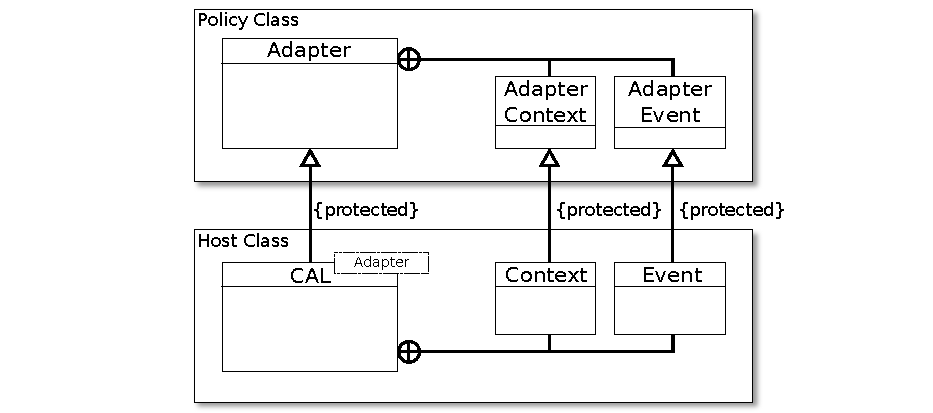
\includegraphics[width=\textwidth]{graphics/40_cal_uml}
  \caption{CAL implemented through policy based design. The adapter is
    configured by a template argument at compile-time. The CAL defines
    the context, event and communication interface. The adapter
    implements the determined interface of the CAL and adapter specific
    context and event classes.}
  \label{fig:cal_uml}
\end{figure}

\noindent The CAL provides all communication methods discussed in
Section~\ref{sec:des:p2p} and~\ref{sec:cal_collective} and context
creation methods discussed in Section~\ref{sec:cal_context}. The
communication policy implements all methods required by the adapter
definition that were discussed in
Section~\ref{sec:impl:policy_interface}.

In addition to communication and context related methods, the CAL
class also provides class interface definitions of the context and
event class. They inherit their functionality from according classes
in the adapter class. Thus, an adapter has to implement an inner
context and an inner event class.  Figure~\ref{fig:cal_uml} shows
context and event of the CAL class inheriting functionality of the
according classes in the adapter class, also in protected
mode. Section~\ref{sec:cal_mpi_adapter} will discuss the
implementation of these adapter specific context and event class
implementation in detail.

%%%%%%%%%%%%%%%%%%%%%%%%%%%%%%%%%%%%%%%%%%%%%%%%%%%%%%%%%%%%%%%%%%%%%%%%%%%%%%%%
%                                                                              %
% POLICY INTERFACE                                                             %
%                                                                              %
%%%%%%%%%%%%%%%%%%%%%%%%%%%%%%%%%%%%%%%%%%%%%%%%%%%%%%%%%%%%%%%%%%%%%%%%%%%%%%%%
% Checked
\subsection{Communication Policy interface}
\label{sec:impl:policy_interface}
An adapter needs to implement the policy interface
determined by the CAL.  The interface was inspired by the
sophisticated MPI language binding for C. Therefore, it is rather low
level to provide the most possible flexibility.  A subset of adapter
methods were chosen to illustrate the interface. A full listing of all
methods should be retrieved from the source code documentation.

\begin{itemize}

  \item Point-to-Point Operation
    \begin{lstlisting}[language=C++, breaklines=false, label={}]
// Adapter Method      
template <typename T_Data, T_Context>      
Event asyncSendData(const T_Data* data,      
                    const unsigned sendCount
                    const VAddr destination,
                    const T_Context context,
                    const unsigned tag); 
    \end{lstlisting}
    
  \item Collective Operation
    \begin{lstlisting}[language=C++, breaklines=false, label={}]
// Adapter Method      
template <typename T_Data, T_Context>      
void gather(const T_Data* sendData,
            const unsigned sendCount,
            const T_Data* recvData,
            const unsigned recvCount,
            const VAddr root,
            const T_Context context);
    \end{lstlisting}

  \item Context Operation
    \begin{lstlisting}[language=C++, breaklines=false, label={}]
// Adapter Method
template <typename T_Context>      
T_Context createContext(const std::vector<VAddr> vAddrs,
                        const T_Context oldContext);
    \end{lstlisting}
  
\end{itemize}

\noindent The adapter interface, only provides a subset
of operations known from MPI or other communication libraries.  Most
of these operations were necessary during the implementation of the
system or used in example applications. The design of interfaces of
more collective operations is left open for future work.


% Addressing of peers
% Checked
\subsection{Mapping to Virtual Addresses}
The design chapter claimed the requirement for an unified address
space to uniquely address peers in a context. The design decision was
to keep it as simple as possible. Therefore, The address space of the
virtual addresses is in the range of natural numbers from 0 to the
number of peers in a context minus one. A adapter needs to map its
own address space into the virtual address space.

% Description Communication operations
% Checked
\subsection{CAL Data Object Interface}
All communication methods are able to transmit data objects from
arbitrary data type defined by the template argument \cpp{T_Data}. The
data object needs to provide a pointer to the data memory and the
number of data elements.  The method \cpp{data()} must return the
pointer and the method \cpp{size()} the number of elements of the
data. C++ Containers of the STL such as \cpp{std::vector} and
\cpp{std::array}~\cite{ref:vector, ref:array} already provide these
methods. Therefore, data can be easily encapsulated into these
containers. Listing~\ref{lst:cal_async_send} shows the implementation of
the \cpp{asyncSend()} method of the CAL. It shows the usage of the
discussed data object interface.  The object \cpp{sendData} with data
type \cpp{T_Data} provides both functions claimed by the
interface. Utilizing \cpp{sendData.data()} and \cpp{sendData.size()}
fulfills the interface requirements of the communication policy
claimed in Section~\ref{sec:impl:policy_interface}.

\begin{lstlisting}[language=C++, breaklines=false, label={lst:cal_async_send}]
// Communication Abstraction Layer Method
template <typename T_Data>
Event asyncSend(const VAddr destVAddr, 
                const Tag tag, 
                const Context context, 
                const T_Data& sendData){

  return Event(
    CommunicationPolicy::asyncSendData(
      sendData.data(),
      sendData.size(), 
      destVAddr, 
      context, 
      tag
      
    )
      
  );

}
\end{lstlisting}

% Description Communication operations
% Checked
\subsection{Reduce Operation interface}
A reduce operation uses a binary operator to reduce a set
of objects of several peers. The C++ STL allready provides a handfull of binary
functions in the ``functional'' header such as \cpp{std::plus},
\cpp{std::multiplies} or \cpp{std::minus}
\cite{ref:functional}. Functions that are not provided by the STL can
be easily created by an C++ struct or class overloading the bracket
operator. Listing~\ref{lst:binary_function} shows such a struct for
the maximum operator.

\begin{lstlisting}[language=C++, breaklines=false, label={lst:binary_function}]
template<typename T_Data>
struct maximum : public std::binary_function<T_Data, T_Data, T_Data> {

  // Bracket operator overloaded with binary operator for maximum
  const T_Data& operator()(const T_Data& x, const T_Data& y) const {
    return x < y? y : x;

  }

};
\end{lstlisting}

\noindent An adapter that implements the reduce operation has to
ensure that it can handle binary operations.  It may exist cases in
which the C++ binary operation has to be transformed to a adapter
specific one.  In these cases, the tranformation logic needs to be
implemented inside the adapter class.  Section~\ref{sec:bin_operator}
discusses the transformation of binary operators by the MPI
adapter.

%%%%%%%%%%%%%%%%%%%%%%%%%%%%%%%%%%%%%%%%%%%%%%%%%%%%%%%%%%%%%%%%%%%%%%%%%%%%%%%%
%                                                                              %
% MPI ADAPTER                                                                  %
%                                                                              %
%%%%%%%%%%%%%%%%%%%%%%%%%%%%%%%%%%%%%%%%%%%%%%%%%%%%%%%%%%%%%%%%%%%%%%%%%%%%%%%%
% Checked
\section{The MPI Adapter as Reference Implementation}
\label{sec:cal_mpi_adapter}

A reference adapter is presented to provide an insight into the
development of an adapter and to provide hints on parts of the adapter
development which should be considered carefully. Furthermore, the
description provides a guideline for the implementation of additional
adapter classes.

The reference adapter implementation is based on MPI as existing
communication library. The adapter acts as a translation or mapping
from the CAL interface to the MPI interface.  MPI (Section
\ref{sec:mpi}) was chosen, because it already provides a lot of
functionality required by the CAL interface without any further
effort. Additionally, it is available on wide range of computing
systems and can be used for free by open source implementations. This
Section will make use of very MPI specific vocabulary. It is assumed
that the reader has a basic knowledge on MPI terminology.

The instantiation of a CAL object, configured by the MPI adapter,
leads to an initialization of the MPI adapter. This initialization
step, creates the initial global context by grouping all peers of
\cpp{MPI\_COMM\_WORLD}.  Furthermore, a mapping from MPI ranks to
virtual addresses for the global context is created in the
\cpp{vAddrMap}. Since, virtual addresses are defined as natural numbers
in the range from zero to the numbers of peers in a context minus one,
the initial \cpp{vAddrMap} contains a one-to-one mapping from virtual
addresses in the global context to MPI ranks in the
\cpp{MPI\_COMM\_WORLD}. The contexts itself are mapped to MPI
Communicators through the \cpp{contextMap}.

%\todo{implement Boost::mpi adapter}

The MPI C language binding is used inside the adapter to address the
message passing interface.  It provides the most general interface to
MPI and can be integrated into a C++ environment.  The interface is
very similar to the adapter interface. Therefore, the implementation
of the adapter interface through MPI routines is not very
complex. Nevertheless shows Listing~\ref{lst:adapter_send} that the
\cpp{asyncSendData} method does not only forward the function call to
the MPI communication method \cpp{MPI_Issend}.  But it also translates
the virtual address \cpp{destination} of the peer to the rank of the
MPI process through the \cpp{vAddrMap} at line~\ref{line:vAddrMap}.
Furthermore, it performs a translation of the context to the MPI
communicator at line~\ref{line:contextMap} through
the~\cpp{contextMap}. Finally, it converts the data type~\cpp{T_Data}
to an MPI data type at line~\ref{line:mpi_datatype}.  The conversion
of data types will be discussed in detail in
Section~\ref{sec:data_type_conversion}.

\begin{lstlisting}[language=C++, breaklines=false, label={lst:adapter_send},escapechar=|]
// Adapter Method
template <typename T_Data, typename T_Context>      
Event asyncSendData(const T_data* const data, 
                    const unsigned count, 
                    const Vaddr destination, 
                    const T_Context context, 
                    const unsigned msgType){    

  // Translation of vaddr to rank
  int destRank      = vAddrMap[context][destVaddr];|\label{line:vAddrMap}|

  // Translation of context to MPI Communicator
  MPI_Comm comm     = contextMap[context];|\label{line:contextMap}|

  // Conversion from T_Data to MPI data type
  MPI_Datatype type = ToMPIDatatype<T_Data>::type;|\label{line:mpi_datatype}|

  // MPI specific send operation                                                                            
  MPI_Request request; 
  MPI_Issend(const_cast<T_Data*>(data), 
             count, 
             type,
             destRank, 
             msgType,
             comm,
             &request);

  // Create and return event
  return Event(request);                                                                                                       

}  
\end{lstlisting}

\noindent The remaining adapter methods are implemented in a similar
manner, except for the reduce operation. Since the CAL interface
accepts, arbitrary binary operators for reducing data, the MPI adapter
need to be able to handle these
operators. Section~\ref{sec:bin_operator} covers the conversion of C++
binary operators to operators that are utilized in MPI.

%%%%%%%%%%%%%%%%%%%%%%%%%%%%%%%%%%%%%%%%%%%%%%%%%%%%%%%%%%%%%%%%%%%%%%%%%%%%%%%%
%                                                                              %
% BINARY OPERATOR                                                              %
%                                                                              %
%%%%%%%%%%%%%%%%%%%%%%%%%%%%%%%%%%%%%%%%%%%%%%%%%%%%%%%%%%%%%%%%%%%%%%%%%%%%%%%%
% Checked
\subsection{Binary Operator}
\label{sec:bin_operator}

MPI provides built-in support for binary operations by two
approaches. The simplest approach, is the direct usage of predefined
binary MPI operators~\cite{ref:mpi_bin_op}. But, since the system user
should not use MPI operators directly, the CAL could wrap all
available MPI operators in a struct of static const expressions like
shown in Listing~\ref{lst:mpi_bin}.  The CAL could forward these
structs to the user of the system and the user could select from these
binary operators.  For example would a reduction by accumulation use
the \cpp{BinaryOperations::SUM} operator.

\begin{lstlisting}[language=C++, caption={A small collection of binary operators by transformed MPI operations to static constexpression }, label=lst:mpi_bin]
struct BinaryOperations { 
  static constexpr BinaryOperation MAX = MPI_MAX; 
  static constexpr BinaryOperation MIN = MPI_MIN; 
  static constexpr BinaryOperation SUM = MPI_SUM; 
  static constexpr BinaryOperation PROD = MPI_PROD; 
  ...

};
\end{lstlisting}


\noindent This approach has the downside that only twelve predefined
operators exist, restricting the application on this limited set of
operators. Therfore, MPI provides the possibility to create abitrary
binary operators with the \cpp{MPI\_Op\_create} function.  The source
code for transforming abitrary binary operators to binary MPI
operators was taken over from the boost::mpi project
\cite{ref:boost_mpi} and was adapted for the needs of the MPI adapter.
Listing \ref{lst:mpi_bin2} shows the transformation of the binary C++
operator \cpp{op} from type \cpp{T\_BinaryOperation} with data type
\cpp{T\_Data} to \cpp{MPIoperator} from type {MPI\_Op}.  After the
transformation, the MPI operator can be retrieved by and used by all
MPI routines that are using binary operators through
\cpp{MPIOperator.getOperator()}.

\begin{lstlisting}[language=C++, caption={ }, label=lst:mpi_bin2]
// Binary C++ operator
T_BinaryOperator op;  
  
// Transformation of binary operator
toMPIOperator<T_Data, T_BinaryOperator> MPIOperator(op);

// Retrieve binary MPI operator
MPIOperator.getOperator()
\end{lstlisting}

\noindent The second approach is essentially more flexible as the
first one. Thus, it was chooses to implement binary operations for the
MPI adapter.

%%%%%%%%%%%%%%%%%%%%%%%%%%%%%%%%%%%%%%%%%%%%%%%%%%%%%%%%%%%%%%%%%%%%%%%%%%%%%%%%
%                                                                              %
% DATA TYPE CONVERSION                                                         %
%                                                                              %
%%%%%%%%%%%%%%%%%%%%%%%%%%%%%%%%%%%%%%%%%%%%%%%%%%%%%%%%%%%%%%%%%%%%%%%%%%%%%%%%
% Checked
\subsection{Data Type Conversion}
\label{sec:data_type_conversion}
On the one hand, MPI predefines primitive data types, but on the other hand also provides 
 the possibility to define data structures based
upon sequences of the MPI primitive data types. These user defined data
structures are called derived data types. Usually, primitive data
types are contiguous. But, derived data types allow you to specify
non-contiguous data in a comfortable manner and to treat it as though
it was contiguous.  Therefore, more complex data types (e.g structs or
classes) can be transformed into derived data types. The exchange
of complex data types was not necessary in the development of the
system based on examples of section \ref{sec:gol_imp}. Therefore, the
implementation was focused on the transformation of primitive data
types.  But nevertheless, a transformation is available in the
boost::mpi \cite{ref:boost_mpi} implementation. Thus switching to
boost::mpi or adopting their source code would solve this problem
without any further effort.

The primitive C++ data types can be mapped directly to primitive MPI
data types. By the fact, that MPI data types are defined by C macros,
a C++ data type need to be converted to an integer number. The
conversion is implemented by the concept of type traits
\cite{ref:type_trait}.  Type traits are classes that obtain
characteristics of types in the form of compile-time constant values.

The function of the type trait is the transformation of primitive C++
data types to primitive MPI data types.  In
Listing~\ref{lst:mpi_trait1} a template struct defines the default
behaviour of the type trait. The struct defines a static const
expression \cpp{type}, which is set to a fixed MPI data type. The
template argument \cpp{T_Data} is the primitive C++ data type that
should be transformed. The default struct will transform arbitrary
data types \cpp{T_Data} to the \cpp{MPI\_CHAR} data type. The MPI data
type of \cpp{T_Data} can be retrieved by
\cpp{ToMPIDatatype<T_Data>::type}.


\begin{lstlisting}[language=C++, label=lst:mpi_trait1]
  template<typename T_Data> 
  struct ToMpiDatatype { 

    static constexpr MPI_Datatype type = MPI_CHAR; 

  };
\end{lstlisting}

\noindent The template in Listing \ref{lst:mpi_trait2} is an explicit
specialization of the default template in Listing
\ref{lst:mpi_trait1}. In this case, a specialization for the C++ data
type \cpp{int}, which will be transformed to the \cpp{MPI\_INT} data type.  Thus,
each transformation of a primitive C++ data type need to be defined
by its own specialization template, assumed that a corresponding
MPI data type exists.

\begin{lstlisting}[language=C++, label=lst:mpi_trait2]
  template<>
  struct ToMPIDatatypes<int> { 

    static constexpr MPI_Datatype type = MPI_INT; 

  };
\end{lstlisting}

\noindent The communication operations within the adapter uses the type trait to
transform the data types of the input and output data, by querying the
type trait. Listing \ref{lst:mpi_trait3} provides an example for the conversion 
of the C++ data type \cpp{int}.

\begin{lstlisting}[language=C++, label=lst:mpi_trait3]
  MPI_Datatype type = ToMPIDataType<int>::type;
\end{lstlisting}

%%%%%%%%%%%%%%%%%%%%%%%%%%%%%%%%%%%%%%%%%%%%%%%%%%%%%%%%%%%%%%%%%%%%%%%%%%%%%%%%
%                                                                              %
% CONTEXT EVENT MPI ADAPTER                                                    %
%                                                                              %
%%%%%%%%%%%%%%%%%%%%%%%%%%%%%%%%%%%%%%%%%%%%%%%%%%%%%%%%%%%%%%%%%%%%%%%%%%%%%%%%
% Checked
\subsection{MPI Adapter Specific Event Implementation}
The MPI adapter specific event utilizes the MPI non-blocking testing
features. In the MPI world, a non-blocking function provides a request
object, which is the handle to verify the state of the
function. Listing~\ref{lst:mpi_event} shows the \cpp{Event}
implementation of the MPI adapter.  The wait method is implemented by
a \cpp{MPI\_Wait} on the request. The ready methods checks with
\cpp{MPI\_Test} whether the function has already finished.


\begin{lstlisting}[language=C++, label=lst:mpi_event]
class Event {
  public:

  Event(MPI_Request request) : request(request){
    
  }
  
  ~Event(){
    
  }

  void wait(){
    MPI_Status status;
    MPI_Wait(&request, &status);
    
  }

  bool ready(){
    int flag = 0;
    MPI_Status status;
    MPI_Test(&request, &flag, &status);
    return bool(flag);
    
  }
  
  private:
  
  MPI_Request request;
};  
\end{lstlisting}

%%%%%%%%%%%%%%%%%%%%%%%%%%%%%%%%%%%%%%%%%%%%%%%%%%%%%%%%%%%%%%%%%%%%%%%%%%%%%%%%
%                                                                              %
% GRAPH IMPLEMENTATION                                                         %
%                                                                              %
%%%%%%%%%%%%%%%%%%%%%%%%%%%%%%%%%%%%%%%%%%%%%%%%%%%%%%%%%%%%%%%%%%%%%%%%%%%%%%%%
% Checked
\section{Graph Based on the Boost Graph Library}
Section \ref{sec:graph} introduced a graph interface.  This graph
interface is implemented on basis of an existing graph library as
back-end. A wide range of graph libraries such as \cite{ref:lemon,
  ref:boost_bgl, ref:igraph, ref:ogdf} were considered as back-end
libraries.  But since, the boost project is closely related to the STL
, the \emph{Boost Graph Library} \cite{ref:boost_bgl}, short \emph{BGL}, was
selected as graph back-end library.  While the BGL provides a powerful
interface and a wide range of graph algorithms, just a small subset of
this functionality is really necessary for the purposes of this
work. Therefore, the BGL is wrapped inside a graph class providing
common graph functionality.  The graph class provides all claimed
methods discussed in design section \ref{sec:graph}, but the methods
are handled by the Boost Graph Library.


%%%%%%%%%%%%%%%%%%%%%%%%%%%%%%%%%%%%%%%%%%%%%%%%%%%%%%%%%%%%%%%%%%%%%%%%%%%%%%%%
%                                                                              %
% PROPERTIES                                                                   %
%                                                                              %
%%%%%%%%%%%%%%%%%%%%%%%%%%%%%%%%%%%%%%%%%%%%%%%%%%%%%%%%%%%%%%%%%%%%%%%%%%%%%%%%
% Checked
\subsection{Vertices Annotated by Properties}

A graph can be anotated by properties. These objects are used to
describe vertices and edges with simulation specific information, like
it was discussed in Section~\ref{sec:graph}. Vertices and edges are
configured by properties at compile-time through a template
parameter. In the wrapper graph implementation, vertices and edges are
represented by the property itself. The BGL refers to vertices and
edges by indices of integer numbers, whereby properties of this
vertices can be queried from so called property maps.

The implementation of a property is a struct or a class with arbitrary
content. It needs to provide an \cpp{id} member variable or inherit
from \cpp{SimpleProperty}. This \cpp{id} is used to create an internal
connection of the property to the vertex index of the BGL.  The most
simple property is a struct only containing the \cpp{id}, like
presented in listing \ref{lst:property}. This property is predefined
in the graph header. It is used as default when the graph is
not configured by a certain property.

\begin{lstlisting}[language=C++, label=lst:property]
struct SimpleProperty {

    SimpleProperty() : id(0) {

    }
    
    SimpleProperty(ID id) : id(id) {

    }

    // Vertex id refers to BGL vertex index
    unsigned id;
};
\end{lstlisting}

\noindent Requesting the vertices of the graph, returns a vector with
all vertices of the graph. But, that vector is actually a list of
vertex properties in the context of the BGL, whereby every property is
connected by its id to the internal BGL graph. This connection is
transparent for the the system user. Hence, the user does not have to
care about it.

%%%%%%%%%%%%%%%%%%%%%%%%%%%%%%%%%%%%%%%%%%%%%%%%%%%%%%%%%%%%%%%%%%%%%%%%%%%%%%%%
%                                                                              %
% CREATION OF A GRAPH                                                          %
%                                                                              %
%%%%%%%%%%%%%%%%%%%%%%%%%%%%%%%%%%%%%%%%%%%%%%%%%%%%%%%%%%%%%%%%%%%%%%%%%%%%%%%%
% Checked
\subsection{Creation of a Graph}
A graph is created by a list of edge descriptors and a list of
corresponding vertices. An edge descriptor is the tuple of source
vertex, destination vertex and the connecting edge. The list of edge
descriptors can also be generated by a graph
generator. Listing~\ref{lst:graph} shows the creation of a graph from
a hypercube topology with three dimensions.

\begin{lstlisting}[language=C++, label=lst:graph]
// Definition of EdgeDescriptor
typedef std::tuple<Vertex, Vertex, Edge> EdgeDescriptor;
const unsigned nDimensions = 3;

// Create vertex and edge vectors
std::vector<Vertex> vertices;
std::vector<EDesc> edges = Topology::hypercube<Graph>(nDimensions, vertices);

// Create graph by edges and vertices
Graph graph(edges, vertices);

\end{lstlisting}

\noindent A set of generators of commonly used graph topologies is already
implemented (Figure \ref{fig:topologies}).  This set of generators
covers fully connected topology, star topology, n-dimensional
hypercube topology and n-dimensional grid topology.  These generators
are parametrizable by number of vertices and/or dimension.  The
functions that generate a topology have the advantage that they can be
reused in different applications with same communication topology.

\begin{figure}[H]
  \centering
  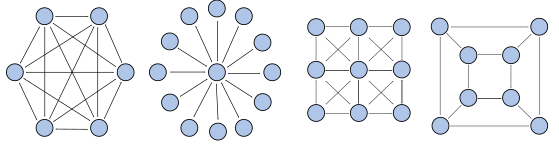
\includegraphics[width=\textwidth]{graphics/40_topologies}
  \caption{Set of already implemented graph generators. Nevertheless,
  abitrary graphs can be generated by user defined generator functions.}
  \label{fig:topologies}
\end{figure}

%%%%%%%%%%%%%%%%%%%%%%%%%%%%%%%%%%%%%%%%%%%%%%%%%%%%%%%%%%%%%%%%%%%%%%%%%%%%%%%%
%                                                                              %
% CREATION OF SUBGRAPHS                                                        %
%                                                                              %
%%%%%%%%%%%%%%%%%%%%%%%%%%%%%%%%%%%%%%%%%%%%%%%%%%%%%%%%%%%%%%%%%%%%%%%%%%%%%%%%
% Checked
\subsection{Creation of a Subgraph}
The creation of a subgraph plays an important role for collective
operations on a subset of graph vertices by the GVON. A subgraph can
be created from its supergraph by a subset of its vertices.  Subgraph
creation is utilized as an equivalent to the creation of sub contexts
in the CAL. Collective operations on this subgraph only consider
vertices within this subgraph. The BGL provides already built-in support
for subgraphs. Listing~\ref{lst:subgraph} shows the creation of the
subgraph from the graph.

\begin{lstlisting}[language=C++, label=lst:subgraph]
  // Creation of a subgraph
  Graph& subGraph = graph.createSubGraph(subGraphVertices);
  
\end{lstlisting}

\noindent A created subgraph is linked to its supergraph, whereby each graph
holds a list of its subgraphs. The connection of super and subgraph is
important for the context creation in collective operations in section
\ref{sec:gvon_impl}, because the announcement of a subgraph considers
first of all the context of the supergraph. Figure
\ref{fig:subgraph_creation} shows the creation of a two-dimensional
hypercube subgraph from a three dimensional hypercube supergraph.

\begin{figure}[H]
  \centering
  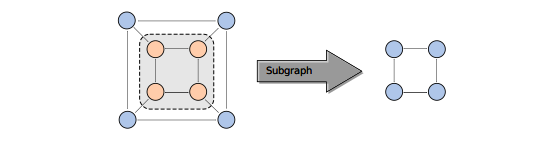
\includegraphics[width=\textwidth]{graphics/40_subgraph_creation}
  \caption{Inner vertices of a three-dimensional hypercube graph are 
  transformed to a two-dimensional hypercube subgraph. Both graphs
  stay in connection by the BGL.}
  \label{fig:subgraph_creation}
\end{figure}

%%%%%%%%%%%%%%%%%%%%%%%%%%%%%%%%%%%%%%%%%%%%%%%%%%%%%%%%%%%%%%%%%%%%%%%%%%%%%%%%
%                                                                              %
% GRAPH BASED VIRTUAL OVERLAY NETWORK                                          %
%                                                                              %
%%%%%%%%%%%%%%%%%%%%%%%%%%%%%%%%%%%%%%%%%%%%%%%%%%%%%%%%%%%%%%%%%%%%%%%%%%%%%%%%
% Checked
\section{Graph-Based Virtual Overlay Network}
\label{sec:gvon_impl}
The GVON was introduced as a combination
of the graph and CAL. This combination is the connection of graph and CAL
by mappings. These mappings are core components of the GVON and are
constructed by the announcement process. The announcement process
implementation is discussed in Section~\ref{sec:announcement_impl}. In
the following each map provided by the GVON is described:

\begin{itemize}
\item [] The \cpp{vertexMap} is a mapping from a vertex to the virtual
address of its host.  This map is used for all methods
that need to resolv the host of a vertex.

\begin{lstlisting}[language=C++, label=lst:mapping1]
std::map<Graph, std::map<Vertex, VAddr> > vertexMap;
\end{lstlisting}


\item [] The \cpp{graphMap} is a mapping from a graph to its related
context created in the announcement process.  This map is important,
since only the hosts of a graph are able to communicate on basis of
this graph.

\begin{lstlisting}[language=C++, label=lst:mapping2]
std::map<Graph, Context> graphMap;
\end{lstlisting}

\end{itemize}
%% \paragraph*{}
%% \todo{What is the peerMap used for ?}
%% \noindent The \cpp{peerMap} is kind of a reverse mapping of the
%% \cpp{vertexMap}.  This map is a mapping from peers to its hosted
%% vertices for a particular graph.
%% \begin{lstlisting}[language=C++, label=lst:mapping3]
%% std::map<Graph, std::map<VAddr, std::vector<Vertex>> > peerMap 
%% \end{lstlisting}

\noindent Listing \ref{lst:comm_gvon} shows the \cpp{asyncSend} method of the
GVON. The vertex is translated to its hosts virtual address in line
\ref{line:gvon_async_send1}. The graph is translated to its context
in line \ref{line:gvon_async_send2}.
\begin{lstlisting}[language=C++, label=lst:comm_gvon,escapechar=|]
// Graph-Based Virtual Overlay Network Method  
template <typename T_Data>
Event asyncSend(Graph& graph, 
                const Vertex destVertex, 
                const Edge edge, 
                const T_Data& data){ 

  // Retrieve host virtual address of destVertex in graph
  VAddr destVAddr = vertexMap[graph][destVertex];|\label{line:gvon_async_send1}|

  // Retrieve context of the graph
  Context context = contextMap[graph];|\label{line:gvon_async_send2}|

  // Use CAL to send data
  return cal.asyncSend(destVAddr, edge.id, context, data);

}
\end{lstlisting}

\noindent Collective operations also utilize the GVON mappings, but their
implementations are far more complex. These implementations will be
discussed in detail in Section~\ref{sec:gvon_collective}.


%%%%%%%%%%%%%%%%%%%%%%%%%%%%%%%%%%%%%%%%%%%%%%%%%%%%%%%%%%%%%%%%%%%%%%%%%%%%%%%%
%                                                                              %
% ANNOUNCEMENT PROCESS                                                         % 
%                                                                              %
%%%%%%%%%%%%%%%%%%%%%%%%%%%%%%%%%%%%%%%%%%%%%%%%%%%%%%%%%%%%%%%%%%%%%%%%%%%%%%%%
% Checked
\subsection{Announcement Process of Graphs}
\label{sec:announcement_impl}

The GVON interface provides an announcement method for the
construction of the mapping from vertices to peers of a context in the
\cpp{vertexMap} and the mapping from graphs to new created contexts in the
\cpp{graphMap}.  The method takes a pair of a graph and a vector of vertices
as input arguments. This means that the peer, calling the announce
method, wants to host these vertices of the graph.  It is a collective
operation of all the peers that want to take part on the communication
of this graph.

These peers need to create an exclusive context for
themselves, which only contains hosts of the graph that will be
announced.  Therefore, the most general context of the hosts, possibly
including more peers, has to be determined.  The overall most general
context is the global context of all peers in the network, but in some
cases exists also a context with less peers.  This is either the
context of the graph or the context of the supergraph, if these graphs
were already announced.

This most general context is used to gather the number of hosted
vertices of each host and to create new context that only contains
peers which host at least one vertex. The graph is mapped to this new
context in the \cpp{graphMap}.

Furthermore, is this new context used for announcing the hosted
vertices of each host through a allGather operation. Such that,
each host can update its \cpp{vertexMap} for this context.

%%%%%%%%%%%%%%%%%%%%%%%%%%%%%%%%%%%%%%%%%%%%%%%%%%%%%%%%%%%%%%%%%%%%%%%%%%%%%%%%
%                                                                              %
% COLLECVITE OPERATIONS LOCALLY                                                %
%                                                                              %
%%%%%%%%%%%%%%%%%%%%%%%%%%%%%%%%%%%%%%%%%%%%%%%%%%%%%%%%%%%%%%%%%%%%%%%%%%%%%%%%
% Checked
\subsection{Collective Operations on Graphs}
\label{sec:gvon_collective}

Because hosts manage potentially more than one vertex, a host has to
perform the collective operation locally for its hosted vertices
first. This means, that data of each hosted vertex has to be collected
locally until the collective operation of the CAL can be performed.
The implementation is a bit tricky since the data objects are from an
arbitrary data type. In the following the collector of a GVON
collective is described:


\begin{itemize}
\item []
  The data of the hosted vertices is collected in a collector object
  until all hosted vertices of this host have terminated their
  collective operation.  The collector is a templated static object
  from type \cpp{std::vector<T_Data>}. Such an collector will
  by created for each data type \cpp{T_DATA}.
  \begin{lstlisting}[language=C++, label=lst:static_collective]
// Type dependent instanciation of the collector
static std::vector<T_Data> collector;
  \end{lstlisting}

\item [] Since, in some cases the resulted data is received by a root vertex, the host of
the root vertex deposits the receive object pointer.
(Listing~\ref{lst:collective}).

\begin{lstlisting}[language=C++, label=lst:root]
// Receive object pointer of root host
static T_Data* rootRecvData;

\end{lstlisting}

\item [] Each call of a collective operation is collecting the data of the
  calling vertex by the collector.  In
  case the the root vertex is calling the operation, the receive pointer
  of the root vertex is stored.
  \begin{lstlisting}[language=C++, label=lst:collecting]
// Collection of vertex data
collector.push_back(vertexData);
  \end{lstlisting}

\end{itemize}

%A peer could try to mix the execution of collective operations of
%several graphs. But, it is only one collective per pair of a graph and
%a vertex allowed concurrently. To ensure that, the amount of already
%executed collective operations per vertex on a graph is counted.  Is
%this count at the beginning of a collective greater than zero, then
%the collective execution is aborted by an exception.

\noindent If the last vertex terminates its collective operation, the
operation is executed locally and then forwarded to the CAL
interface. The CAL executes the collective operation among all
other hosts of the graph and returns the result. For collectives like
gather, the resulting data is reorder such that the GVON returns the
data in vertex id order. Finally, the result is written to the receive
pointer of the root vertex.


%%%%%%%%%%%%%%%%%%%%%%%%%%%%%%%%%%%%%%%%%%%%%%%%%%%%%%%%%%%%%%%%%%%%%%%%%%%%%%%%
%                                                                              %
% GAME OF LIFE IMPLEMENTATION                                                  %
%                                                                              %
%%%%%%%%%%%%%%%%%%%%%%%%%%%%%%%%%%%%%%%%%%%%%%%%%%%%%%%%%%%%%%%%%%%%%%%%%%%%%%%%

\section{Implementing a Game of Life}
\label{sec:impl:gol}
The Game of Life simulation was implemented to show the developed
system in a real world scenario. The set of implemented rules based on
\cite{ref:gol_rules} is listed in the following:

\begin{enumerate}
\item Any live cell with fewer than two live neighbours dies, as if caused by under-population.
\item Any live cell with two or three live neighbours lives on to the next generation.
\item Any live cell with more than three live neighbours dies, as if by overcrowding.
\item Any dead cell with exactly three live neighbours becomes a live cell, as if by reproduction.
\end{enumerate}

%%%%%%%%%%%%%%%%%%%%%%%%%%%%%%%%%%%%%%%%%%%%%%%%%%%%%%%%%%%%%%%%%%%%%%%%%%%%%%%%
%                                                                              %
% CONFIGURATION AND INITIALIZATION OF GOL                                      %
%                                                                              %
%%%%%%%%%%%%%%%%%%%%%%%%%%%%%%%%%%%%%%%%%%%%%%%%%%%%%%%%%%%%%%%%%%%%%%%%%%%%%%%%
% Checked
\subsection{Configuration and Initialization of Game of Life}
The following source code describes necessary steps to configure and
initialize the system before starting the communication of GoL. The
source code uses the presented MPI adapter, GoL graph and
Cell property. It should demonstrate the general program flow and be
the foundation for usage in other simulation applications.

\begin{enumerate}

\item \textbf{Configuration}
\begin{enumerate}

\item Configure the CAL
  
  The target system is a cluster providing MPI as communication
  library. Therefore, the CAL is configured by the reference MPI adapter
  described in Section~\ref{sec:cal_mpi_adapter}. The adapter provides
  type definitions for the virtual address, event and context that are
  necessary for later usage:

  \begin{lstlisting}[language=C++, label=lst:conf_cal, caption={}]
// Configure CAL
typedef CommunicationPolicy::MPI                  Mpi;
typedef CommunicationAbstractionLayer<Mpi>        MpiCAL;
typedef typename MpiCAL::VAddr                    VAddr;
typedef typename MpiCAL::Event                    Event;
  \end{lstlisting}

\item Configure graph

  The graph is configured with the properties \cpp{Cell} for vertices
  (Listing~\ref{lst:gol_cell}) and \cpp{SimpleProperty} for edges. It
  provides type definitions for vertex, edge and edge descriptor:

  \begin{lstlisting}[language=C++, label=lst:conf_graph, caption={}]
// Configure graph
typedef Graph<Cell, SimpleProperty>               GoLGraph;
typedef typename GoLGraph::Vertex                 Vertex;
typedef typename GoLGraph::Edge                   Edge;
typedef typename GoLGraph::EdgeDescriptor         EDesc;
  \end{lstlisting}

  The \cpp{Cell} property contains the state information of a cell, and
  inherits from \cpp{SimpleProperty} the vertex id. 31.25 percent of
  all cells are initialized with their state \cpp{isAlive} set to true.  The
  following listing shows the source code of the \cpp{Cell} property.
  
  \begin{lstlisting}[language=C++, label=lst:gol_cell, caption={}]
// Cell property    
struct Cell : public SimpleProperty { 

 Cell() : SimpleProperty(0), isAlive{{0}}, aliveNeighbors(0){ 
          
 }
        
 // Initialization of the cell
 Cell(ID id) : SimpleProperty(id), isAlive{{0}}), aliveNeighbors(0){ 
   unsigned random = rand() % 10000;
   if(random < 3125){ 
     isAlive[0] = 1;
     
   }
   
 }

 // State of the cell
 std::array<unsigned, 1> isAlive;

 // Number of alive neighbors
 unsigned aliveNeighbors;
 
};
\end{lstlisting}

\item Configure GVON

  The GVON is configured by the previously configured \cpp{MpiCAL} and
  \cpp{GoLGraph}

  \begin{lstlisting}[language=C++, label=lst:conf_gvon, caption={}]
// Configure GVON
typedef VirtualOverlayNetwork<GoLGraph, MpiCAL>  GVON;
  \end{lstlisting}

\end{enumerate}

\item \textbf{Initialization}
  \begin{enumerate}
  
  \item Create graph object

    The graph is generated by the predefined graph generator for
    grids. The generator creates a two dimensional grid , while
    diagonal arranged cells are connected (similar to Figure
    \ref{fig:gol_modeling}).

  \begin{lstlisting}[language=C++, label=lst:gol_generator_graph, caption={}]
// STL namespace
using namespace std;

// Generate GoL graph
vector<Vertex> vertices;
vector<EDesc> edges = Topo::gridDiagonal<GoLGraph>(n, vertices);
GoLGraph graph (edges, vertices); 
  \end{lstlisting}

\item Create the CAL and GVON objects

  \begin{lstlisting}[language=C++, label=lst:, caption={}]
// Instanciate CAL and GVON
MpiCAL cal;
GVON gvon(cal);
  \end{lstlisting}

\item Distribute vertices

  The graph vertices are distributed by the round-robin method, which
  is by far no optimal vertex distribution method, but this is not the
  focus of this work.

  \begin{lstlisting}[language=C++, label=lst:gol_distribution, caption={}]
// Distribution of graph by round-robin
Context context = cal.getGlobalContext();
vector<Vertex> hostedVertices = Dist::roundrobin(context, graph);
  \end{lstlisting}

  \noindent Other distribution methods are also possible. Figure
  \ref{fig:gol_mapping} shows two different vertex distributions
  methods.  In the first distribution, hosted vertices are connected
  within the same host, since this reduces communication operations
  with other peers.  In the second distribution every vertex is
  hosted by exactly one peer, representing a case where the graph
  represents exactly the communicating processes.

  \begin{figure}[H]
    \centering
    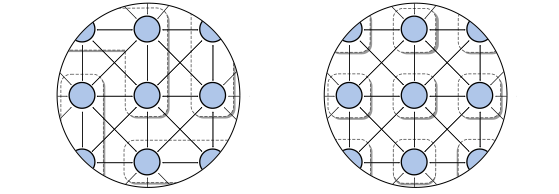
\includegraphics[width=\textwidth]{graphics/40_gol_mapping}
    \caption{Image section of the GoL world. Possible distribution of modelled
      GoL graph. On the left side a peer host a connected set of
      vertices. While, on the right side, every peer hosts exactly one
      vertex.}
    \label{fig:gol_mapping}
  \end{figure}

  \noindent A distribution is possible from one host that hosts all
  vertices to the number of hosts where every host get exactly one
  vertex. Executing an application with more peers than available
  vertices is an interesting case for fault tolerance and load
  balancing.  Additional peers could be used as backup peers, but this
  is left open for future work.  After distribution vertices, every
  peer announces its vertices to the GVON.

\item Announcement of hosted vertices
  \begin{lstlisting}[language=C++, label=lst:gol_announce, caption={\ }]
// Announcement of hosted vertices
gvon.announce(graph, hostedVertices);
  \end{lstlisting}
  \end{enumerate}
\end{enumerate}

%%%%%%%%%%%%%%%%%%%%%%%%%%%%%%%%%%%%%%%%%%%%%%%%%%%%%%%%%%%%%%%%%%%%%%%%%%%%%%%%
%                                                                              %
% COMMUNICATION OF GAME OF LIFE                                                %
%                                                                              %
%%%%%%%%%%%%%%%%%%%%%%%%%%%%%%%%%%%%%%%%%%%%%%%%%%%%%%%%%%%%%%%%%%%%%%%%%%%%%%%%
% Checked
\subsection{Communication of Game of Life}
\label{sec:gol_imp}
Since the utilized GoL rules only require next neighbor communication,
the GoL domain is modeled as a two-dimensional grid with diagonal
connections like in Section~\ref{sec:gol}. Therefore, a GoL cell is
represented by a vertex and neighboring cells are connected by
edges. A cell has to communicate with its neighboring cells. Thereby
it retrieves the neighbor cells state to calculate its own state for
the next time-step.

In the following, the implementation of a single evolution step of GoL
is described. The Communication between vertices of the GoL graph
is handled by the GVON. A host has a list of its hosted vertices it is
responsible for. Therefore, a host has to manage the communication of its
hosted vertices. In the case of GoL, a host has to exchange the state
of its hosted cells with neighboring cells.

First, each host sends the state of its cells to neighboring
cells (Listing \ref{lst:gol_send}). The host retrieves the target
vertex of outgoing edges for a hosted vertex from the graph. After that,
the state of the according cell is transmitted to the target vertices
sequentially in non-blocking mode (Figure
\ref{fig:gol_communication}). Events of the send operation are
collected and checked later for termination.

\begin{lstlisting}[language=C++, label=lst:gol_send, caption={\ }]
// Send state to neighbor cells
for(Vertex myVertex : hostedVertices){
  for(std::pair<Vertex, Edge> outEdge : graph.getOutEdges(myVertex)){

    // Retrieve target vertex
    Vertex targetVertex = outEdge.first;
    Edge   edge         = outEdge.second;

    // Send cell state to neighboring cell
    events.push_back(
      gvon.asyncSend(graph, targetVertex, edge, myVertex.isAlive)
    );

  }

}
\end{lstlisting}

\noindent Second, each host receives state information of
neighboring cells for each of its hosted vertices (Listing
\ref{lst:gol_recv}). The host queries the source vertex of incoming
edges of its hosted vertices from the graph. Afterwards, it receives the
state information from this neighboring source vertex.  The receive
operation is used in blocking mode. So that, all peers are
synchronized afterwards.

\begin{lstlisting}[language=C++, label=lst:gol_recv, caption={\ }]
// Recv state from neighbor cells
for(Vertex myVertex : hostedVertices){
  for(std::pair<Vertex, Edge> inEdge : graph.getInEdges(myVertex)){

    // Retrieve source vertex
    Vertex sourceVertex = inEdge.first;
    Edge   edge         = inEdge.second;

    // Receive cell state of neighboring cell    
    gvon.recv(graph, sourceVertex, edge, sourceVertex.isAlive);

    // Update number of neighbors
    if(sourceVertex.isAlive[0]) { 
      myVertex.aliveNeighbors++;

  }

}
\end{lstlisting}

\noindent Figure \ref{fig:gol_communication} shows the sending process of a host
for each of its hosted vertices.

\begin{figure}[H]
  \centering
  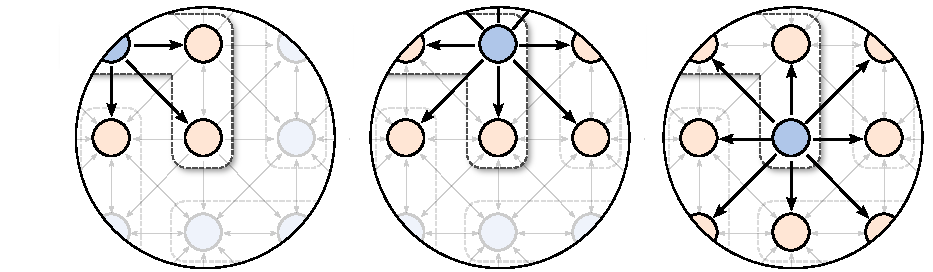
\includegraphics[width=\textwidth]{graphics/40_gol_communication}
  \caption{Image section of the GoL world. A peer sends status information of
    hosted cells to neighboring cells. The communication operations
    are executed sequentially, but non blocking. Receive operations
    behave analog, but in blocking mode.}
  \label{fig:gol_communication}
\end{figure}

\noindent Once all send and receive operations are finished, the peer
updates the state of its hosted cells by the state of their
neighboring cells in dependence of the introduced rules. Finally, the
state information of all cells is gathered by the root vertex (vertex
with id = 0) which prints it to the console for visualization (Listing
\ref{lst:gol_gather}). The next evolution steps will repeat the
previous communication steps until the application is aborted or a
fixed number of evolution steps is reached.

\begin{lstlisting}[language=C++, label=lst:gol_gather, caption={\ } ]
// Gather state by root vertex
for(Vertex myVertex: hostedVertices){
  gvon.gather(root, myVertex, graph, myVertex.isAlive, golGameField);

}
\end{lstlisting}


%%%%%%%%%%%%%%%%%%%%%%%%%%%%%%%%%%%%%%%%%%%%%%%%%%%%%%%%%%%%%%%%%%%%%%%%%%%%%%%%
%                                                                              %
% Implementation N-BODY                                                        %
%                                                                              %
%%%%%%%%%%%%%%%%%%%%%%%%%%%%%%%%%%%%%%%%%%%%%%%%%%%%%%%%%%%%%%%%%%%%%%%%%%%%%%%%
\section{Implementing a N-Body Simulation}
\label{sec:impl:nbody}


The implementation of the N-body simulation, discussed in section
\ref{sec:design:nbody}, does not differ very much from the GoL
implementation with respect to the GVON. Its implementation is
also separated into three phases: configuration, initialization and
communication. The slight differences in implementation details are
described in the following enumeration:

\begin{enumerate}
\item \textbf{Configuration}

  The Graph is annotated by the property
  \cpp{Particle}, containing Particle information mass, velocity and
  location.

\item \textbf{Initialization}

  Since, the chosen N-body algorithm is
  based on an all-to-all communication schema, the communication
  dependencies are described by an fully connected graph.

\item \textbf{Communication}

  Every host sends particle information
  of its hosted vertices to adjacent vertices. In turn, it receives
  particle information from all adjacent vertices. Since, a vertex is
  adjacent to all other vertices, it sends and receives to and from
  all other vertices.
\end{enumerate}

\noindent After each communication step, a host updates the state of
the particles of its hosted vertices.  The communication phase is
repeated for an arbitrary amount of time steps or until the simulation
execution is canceled.

The implemented N-body simulation is completely different from the
presented GoL implementation, but provides similar communication
concepts. Therefore, it was very easy to implement this N-body
simulation by slightly change the GoL source code.


%%%%%%%%%%%%%%%%%%%%%%%%%%%%%%%%%%%%%%%%%%%%%%%%%%%%%%%%%%%%%%%%%%%%%%%%%%%%%%%%
%                                                                              %
% REDISTRIBUTION OF VERTICES                                                   %
%                                                                              %
%%%%%%%%%%%%%%%%%%%%%%%%%%%%%%%%%%%%%%%%%%%%%%%%%%%%%%%%%%%%%%%%%%%%%%%%%%%%%%%%
\section{Redistribution of vertices}

The GVON provides explicit mappings from vertices to peers and from
graphs to contexts. These mappings are changeable during the run-time
of the simulation application.  To show that behavior of the system, a
occupation scenario, where a vertex is changing its host, is
implemented to demonstrate a kind of load balancing at run-time. This
is possible, since hosted vertices are not bound statically to its
hosts.

The scenario is the following: a host occupies or steels a vertex
from another host and henceforward hosts this vertex.  This process
is declared as occupation, because the change of the host is
dictated by the so called master host.

The occupation process start by determining the master host of a
context. The master is the result of a random number modulo the size
of the context. To find a consensus random number in the context,
every host generates an own random number and the consensus random
number is calculated by accumulating all random numbers by a
reduce operation.

Once the master is determined, it defines a occupy vertex of the
graph. This vertex needs to be hosted from another host. Such that,
the master does not occupy a vertex from itself.

The occupy vertex is broadcasted to the set of hosts in the context
and every host in the context checks whether this vertex is contained
in its set of hosted vertices. The host which manages this vertex must
release it, while the master host adds the vertex to its hosted
vertices.

Although, the hosts know the master and the vertex that was occupied,
distribution and announcement process are strictly
separated. Therefore, the host need to reannounce their hosted
vertices of the graph. Even though nothing changed for the most peers.

Figure \ref{fig:gol_remapping} demonstrates the occupation of a
vertex.  The occupied vertex does not need to be adjacent to hosted
vertices of the master host.

  \begin{figure}[H]
    \centering
    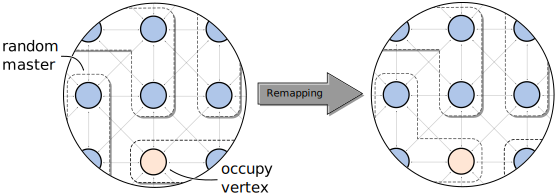
\includegraphics[width=\textwidth]{graphics/40_gol_remapping}
    \caption{Remapping of vertices to peers. A random master peer is
      determined by a consensus random number generation. The master
      dictates the vertex which will be occupied. Vertices of the
      graph are reannounced.}
    \label{fig:gol_remapping}
  \end{figure}

\noindent Even though, this occupation scenario is an simple example, it
shows remapping of vertices at runtime and therefore the power
to establish load balancing and fault tolerance techniques on
top of the system.

\cleardoublepage

%%% Local Variables:
%%% TeX-master: "diplom"
%%% End:
